\documentclass[conference]{IEEEtran}
\IEEEoverridecommandlockouts
% The preceding line is only needed to identify funding in the first footnote. If that is unneeded, please comment it out.
\usepackage[numbers]{natbib}
\usepackage{amsmath,amssymb,amsfonts}
\usepackage{algorithmic}
\usepackage{graphicx}
\usepackage{textcomp}
\usepackage{xcolor}
\def\BibTeX{{\rm B\kern-.05em{\sc i\kern-.025em b}\kern-.08em
    T\kern-.1667em\lower.7ex\hbox{E}\kern-.125emX}}

\begin{document}
\title{Smart concentrated liquidity}

\author{\IEEEauthorblockN{Stefan Duprey}
\IEEEauthorblockA{\textit{SwissBorg} \\
stefan@swissborg.com}
}

\maketitle

\begin{abstract}
Uniswap is the largest decentralized exchange (DEX) and one of cornerstones of Decentralized Finance (DeFi). Uniswap uses liquidity pools to provide Automated Market Making (AMM) functionality. Uniswap can provide more liquidity than its larger, centralized rivals Coinbase and Binance, because of the incentives it gives its liquidity providers to deliver better pricing to traders.\\
Uniswap version 3 is pioneering the new concept of concentrated liquidity feature, which allows the liquidity providers to concentrate their liquidity in a specific price range, leading to an increased capital efficiency compared to the previous v2 version.\\
However, the mathematical relationship between the liquidity position, the amount of assets in that position, and its price range becomes somewhat complex and the corollary to that capital efficiency is an even nastier impermanent loss risk than v2 when the initial price diverges from the initial entry price for the liquidity provision.\\
The ability to concentrate liquidity on uniswap V3 has been designed for people to gain efficiency on the capital they bring, but the key issue there is to find a suitable algorithm to rebalance the liquidity position bounds to maximize volume fees while keeping impermanent loss and rebalancing costs (transaction costs + swapping slippage) low.\\
One has to understand that the provision of liquidity in hyperbolic dexes will loose as soon as the price diverges (upwards or downwards) from where the initial price was when the liquidity was brought.\\
So liquidity provisioning has to be actively monitored. The chosen bounds must be actively managed to encompass the price moves and not get traversed.\\
In a volatile market, finding the right bounds for an optimal trading liquidity concentration is a challenging exercise : one has to find the optimal bounds rebalancing strategy for the perfect trade-off between impermanent loss, swapping costs and swapping volume fees generation.\\
Bullish/bearish market must be avoided at all costs : the market will traverse your bounds and leave you with your liquidity either in full stable coins in a bullish market or in full risky asset in a bearish market.\\
Passive liquidity investing must be seen as, in essence, a mean reverting strategy where the money is made from price fluctuation inside a specified range.\\
An algorithmic detection is therefore a must : one should discriminate markets as rangy, bullish or bearish and apply only passive liquidity provisioning in rangy markets.\\
We here detail the trade-off optimization problem to detect liquidity bounds algorithmically.
\\
\begin{description}
  \item[$\bullet$]Maximize price inside the tightest bounds to earn volume fees (the tighter the bounds, the efficienter the capital)
  \item[$\bullet$] Impermanent loss and swapping slippage costs incurred at each rebalancing have to be minimized
\end{description}
We here give a rebalancing methodology and the optimal matching parameters found by an exhaustive computational backtesting approach.\\
A proper analysis of the rebalancing costs versus fees generation is done.\\
An absolute performance analysis proves that the LP value fluctuation can be very corrosive when the underlying risky drops in value as both impermanent loss and 50\% risky position asset depreciation cumulate.\\
We then propose a new algorithm based on a trend detection signal where the loss in bearish market are mitigating by\\
\begin{description}
  \item[$\bullet$] Either shorting by using Aave money market
  \item[$\bullet$] Or hedging the LP position by buying an option basket for a specific maturity
  \item[$\bullet$] Or just shorting a perpetual according the delta of the LP position value (its sensitivity to the underlying)
\end{description}
\end{abstract}
\section{Building different flavours :market-neutral, long, short}
Simply bringing liquidity in a uniswap v3 position is a risky strategy. In addition to a nasty v3 impermanent loss, you can also incur the depreciation of the long side of the LP position in case of a negative price action for the risky asset.\\
To avoid this double penalty, one has to devise ways to take directional positions (both long and short) and take directional bets to benefit from bearish market stages too.\\
Or simply become market neutral by removing 
\subsection{Neutral leg}
\subsubsection{Configuration}
\begin{figure}[h!]
    \centering
    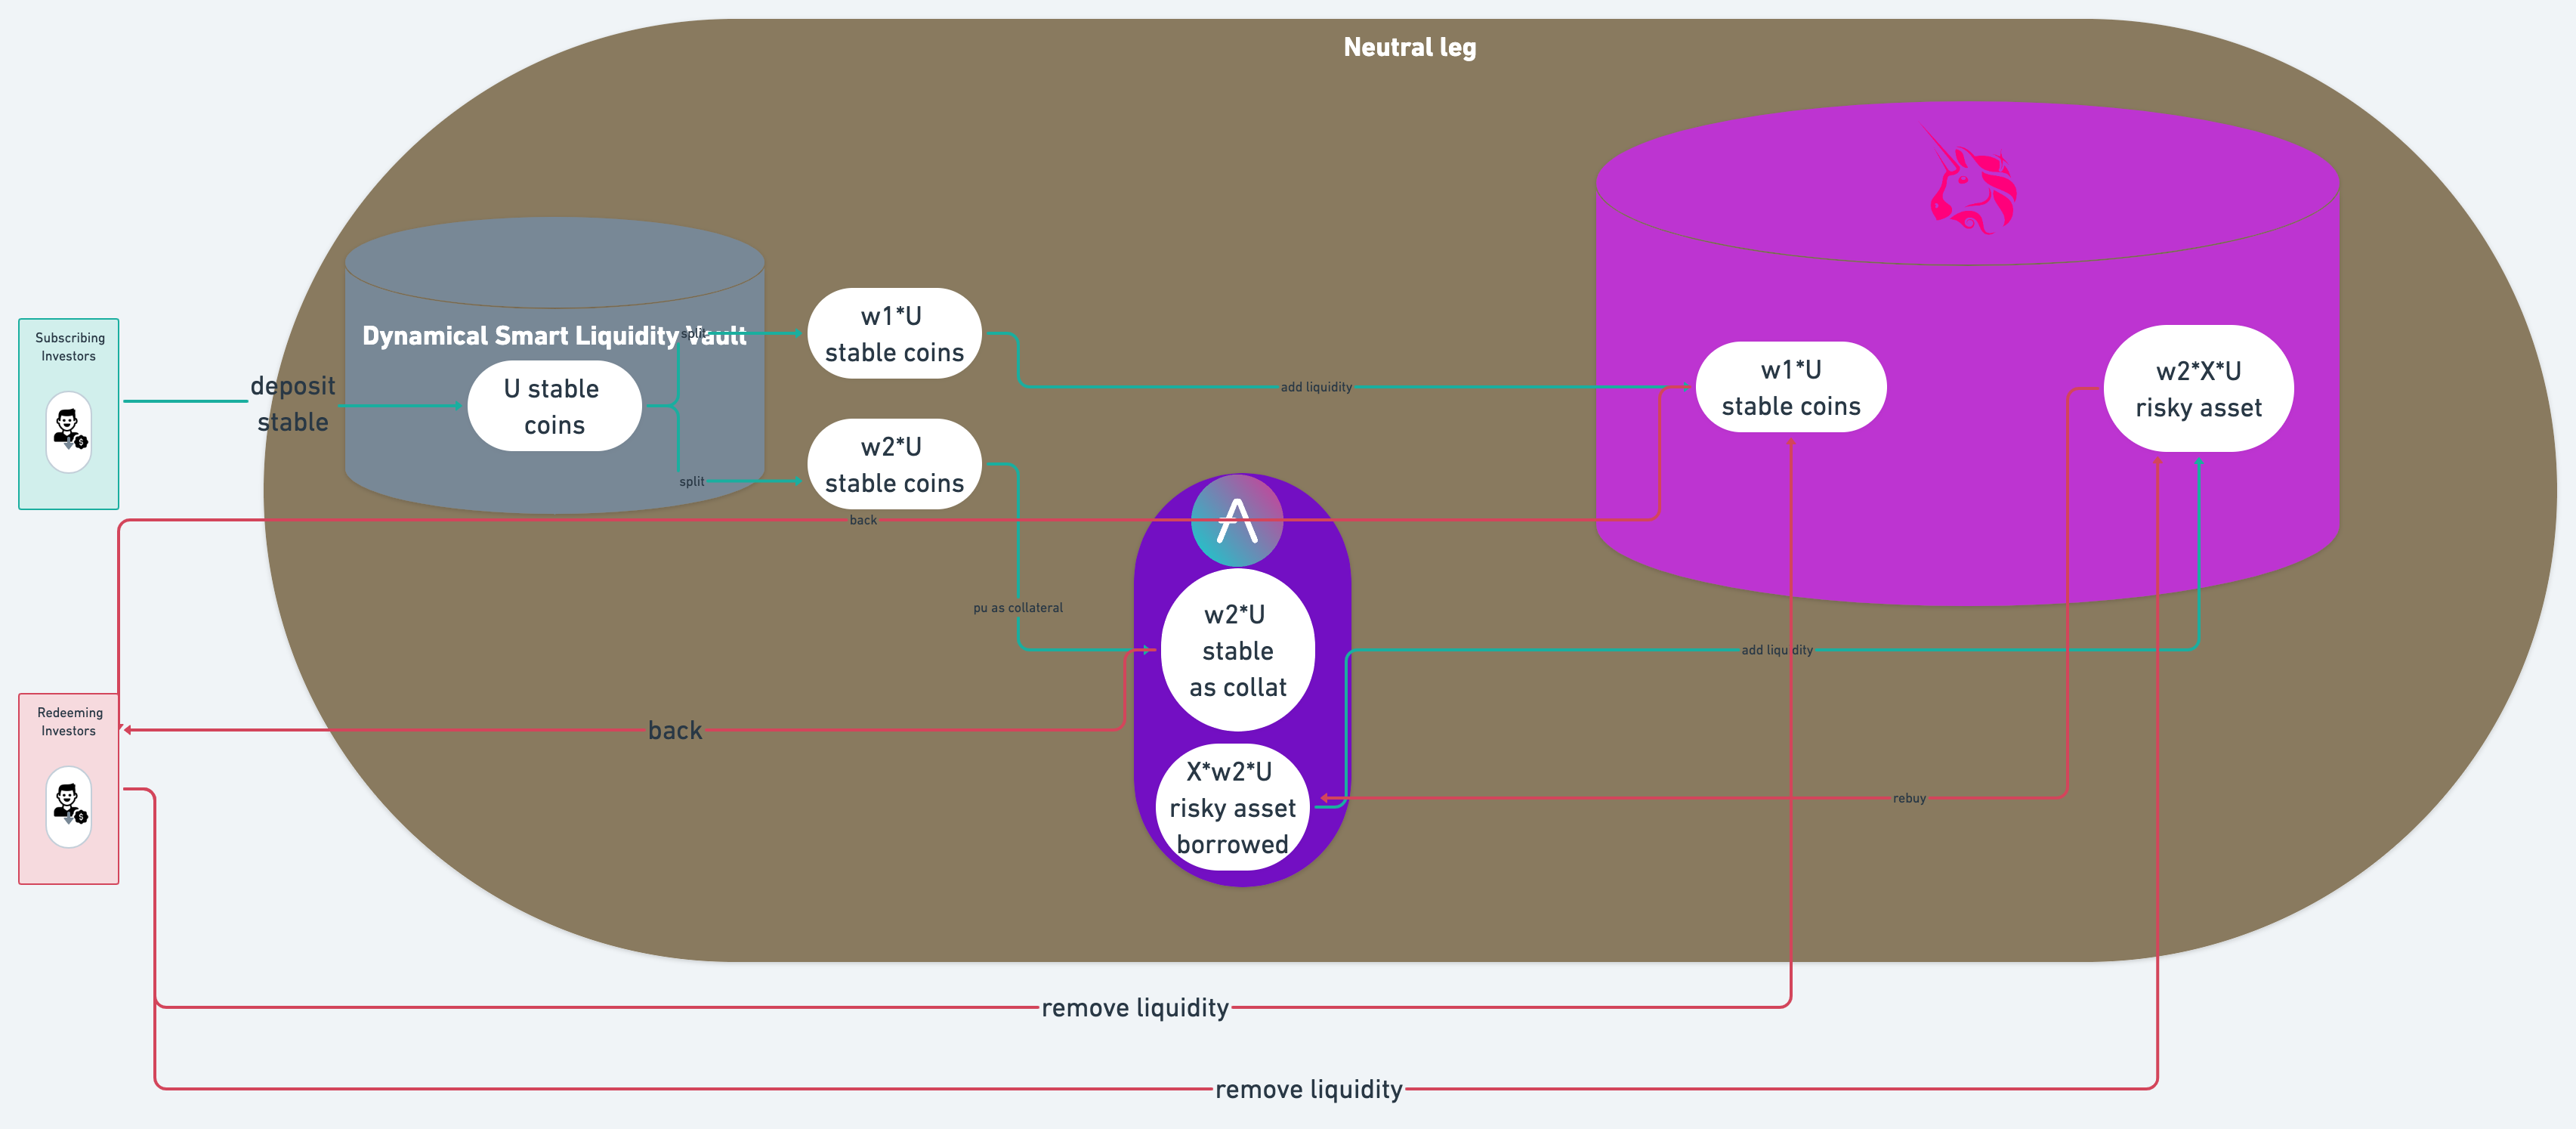
\includegraphics[scale=0.07]{Plots/neutral_leg.png}
    \caption{Neutral}
    \label{fig:neutral_leg}
\end{figure}
The neutral configuration is achieved by using a money market to borrow the risky asset. We enter with a non risky/stable asset and borrow the risky part of the LP position through the money market. This has a cost incurred because of the borrowing on the money market.\\
We enter with an amount $U$ of stable asset.\\
The splitting quantities $\omega_1$ and $\omega_2$ must verify : 
\begin{equation}
\begin{array}{ll}
\omega_1 + \omega_2 = 1\\https://www.overleaf.com/project/63982f2b00b8e4f60c47ea82
\omega_1 * U = X_{risky}*\omega_2 * U\\    
\end{array}
\end{equation}
, where $X_{risky}$ is the risky collateral ratio : the amount of risky asset you can borrow against your stable asset.\\
The solution is given by the splitting quantities :
\begin{equation}
\left\{
\begin{array}{ll}
\omega_1  = \frac{X_{risky}}{1+X_{risky}}\\
\omega_2  = \frac{1}{1+X_{risky}}\\
\end{array}\right.
\end{equation}
\subsubsection{Operation}
To avoid the risk of being liquidated, we will only borrow $X << X_{risky}$ leading to a clearly smaller LP position when compared to the entry size. This will lead to lower yield but a safer strategy.\\
Impermanent loss can be nasty, and we want to have a safe buffer to avoid liquidation.\\
Now that the asset has been borrowed, our position is only subject to the impermanent loss.\\
\subsection{Long/Short legs}
\subsubsection{Long leg}
\begin{figure}[h!]
    \centering
    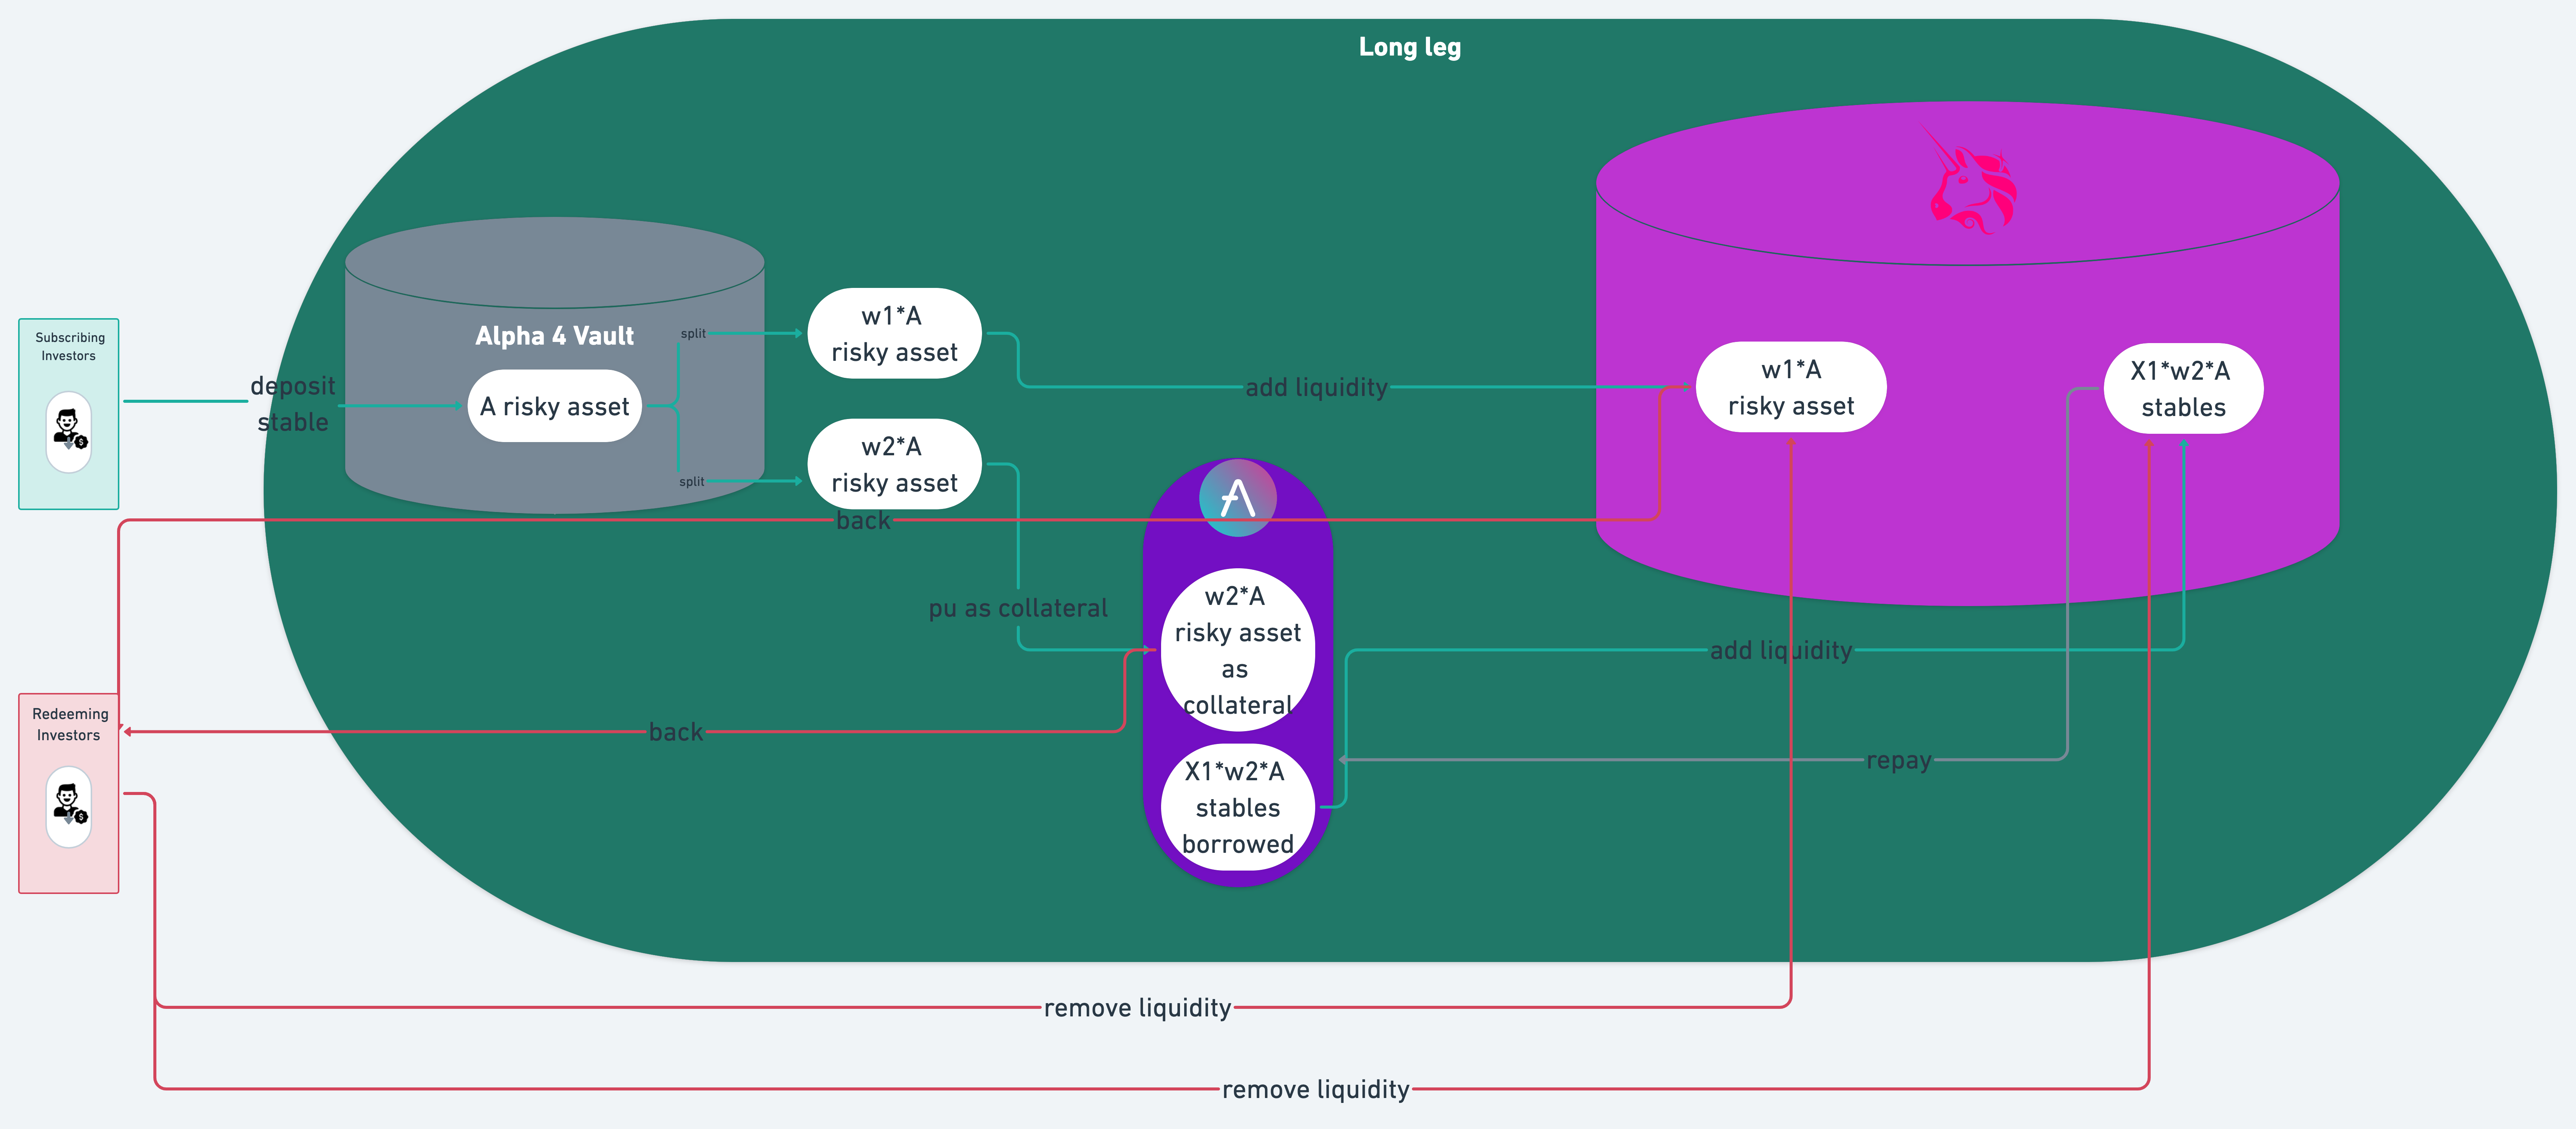
\includegraphics[scale=0.035]{Plots/long_leg.png}
    \caption{Long}
    \label{fig:long_leg}
\end{figure}
The splitting quantities $\omega_1$ and $\omega_2$ must verify : 
\begin{equation}
\begin{array}{ll}
\omega_1 + \omega_2 = 1\\
\omega_1 * A = X_1*\omega_2 * A\\    
\end{array}
\end{equation}
, where $X_1$ is the collateral ratio : the amount of stable coins you can borrow against your Solana.\\
The solution is given by the splitting quantities :
\begin{equation}
\left\{
\begin{array}{ll}
\omega_1  = \frac{X_1}{1+X_1}\\
\omega_2  = \frac{1}{1+X_1}\\
\end{array}\right.
\end{equation}
\subsubsection{Short leg}
\begin{figure}[h!]
    \centering
    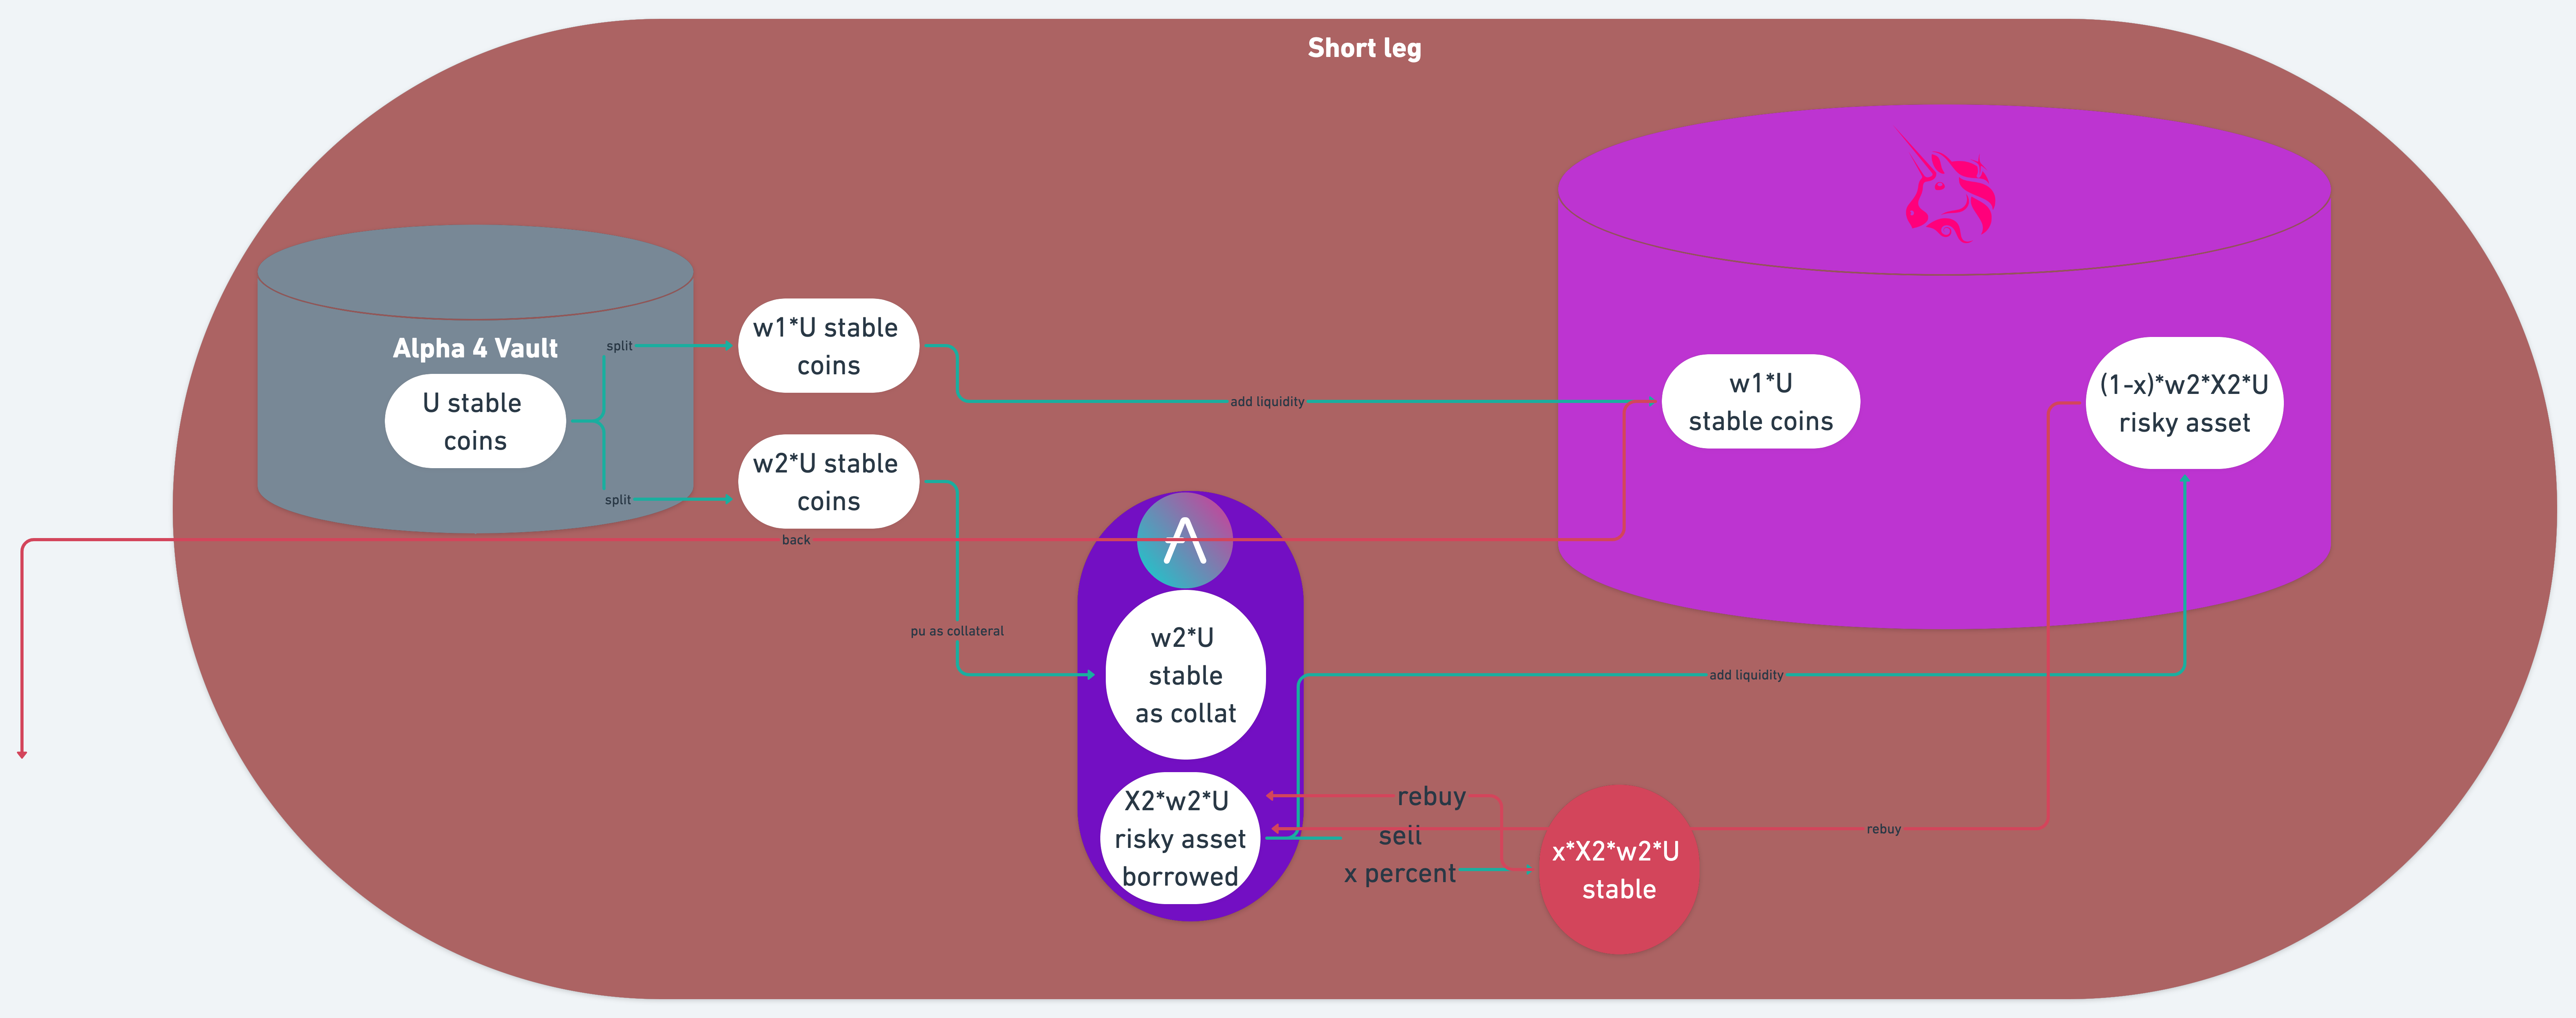
\includegraphics[scale=0.035]{Plots/short_leg.png}
    \caption{Short}
    \label{fig:short_leg}
\end{figure}
The splitting quantities $\omega_1$ and $\omega_2$ must verify : 
\begin{equation}
\begin{array}{ll}
\omega_1 + \omega_2 = 1\\
\omega_1*U = (1-x)*\omega_2*X_2*U\\    
\end{array}
\end{equation}
, where $X_2$ is the collateral ratio : the amount of sols you can borrow against your stable coin and $x$ is the proportion of your borrowed Sols you use to short.\\
The solution is given by fixing the amount you have to short as a function of your liquidity position size $\omega_1$ ($x=f(\omega_1)$):
\begin{equation}
x = \frac{(1-\omega_1)*X2-\omega_1}{(1-\omega_1)*X2}
\end{equation}

\begin{figure}[h!]
    \centering
    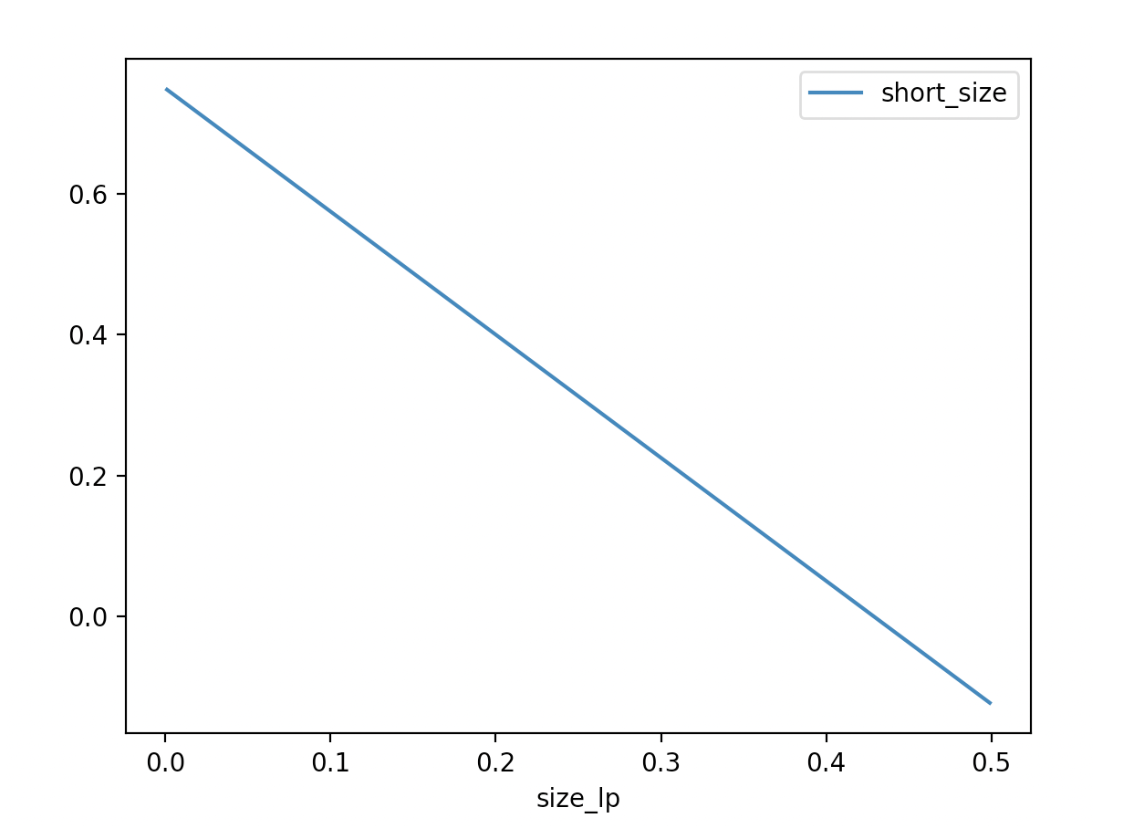
\includegraphics[scale=0.3]{Plots/short_size_as_lp_size.png}
    \caption{Long leg}
    \label{fig:conc_liquidity}
\end{figure}
We can see that the amount of short position we want to have will directly dictate the size of our LP position and therefore the fees we produce.\\
For a LP position of size 0, then $x=X_2$, meaning that we short the whole $\omega_2$ split from our asset.\\
For a LP of maximal size of $\omega_1 = \frac{1}{1+X_2}$ (roughly 55\%), then we have no room left to short : $x=0$.\\
For a LP size in between those bounds, it gives the following short position by noting : ${\text total-short-position} = S $\\
\begin{equation}
\begin{array}{ll}
S= x*(1-\omega_1)X2*U \\
S =  \left((1-\omega_1)*X2-\omega_1 \right)*U\\
\end{array}
\end{equation}\\
where $U$ is the amount of the stable coins at the beginning of the epoch.
The idea is to use that range of shorting size to adapt to our proprietary epoch market indicator by cumulating a long and a short leg simultaneously in an adaptating ratio.\\
By noting : ${\text total-long-position} = L $\ for a long leg.
\begin{equation}
L = A
\end{equation}\\where $A$ is the amount of risky coin at the beginning of the epoch.\\

So according to the risk level from our proprietary indicator for the next epoch, we can taylor the $\frac{short}{long}$ position ratio in a continuous way by allocating specific sizes of risky and numeraire asset:\\
\begin{equation}
\left\{
\begin{array}{lll}
\frac{A}{U} = \left((1-\omega_1)*X2-\omega_1 \right)\text{market neutral} \\
\frac{A}{U} > \left((1-\omega_1)*X2-\omega_1 \right) \text{long overall} \\
\frac{A}{U} < \left((1-\omega_1)*X2-\omega_1 \right)\text{short overall}  \\
\end{array}
\end{equation}
\section{Actively rebalancing your liquidity for a market neutral solution}
Let us here consider the market neutral configuration : we have entered an LP position with a borrowed risky asset and are therefore only subject to the impermanent loss.\\
As demonstrated in the appendix \ref{v3isbad}, V3 impermanent loss can be nasty, and the tighter you encompass your price, the more violent it becomes.\\
We here under propose a quantitative algorithm to dynamically mitigate it.\\
\subsection{Dynamical exiting}
Market making is in essence a very complex topic. Professional traditional finance market makers have advanced algorithmic trading to manage their risk and avoid market trends.\\
Market makers profit only from rangy markets and must exit as soon as a trend takes hold (upward and downward).\\
V3 liquidity provisioning is market making in essence and V3 concentrated liquidity ressembles an order book.\\ 

\subsubsection{Trend exiting signal}
Based on a proprietarly hourly volatilitity/trend detecting signal, we manage to capture trendy versus rangy market hours.\\
\begin{figure}[h!]
    \centering
    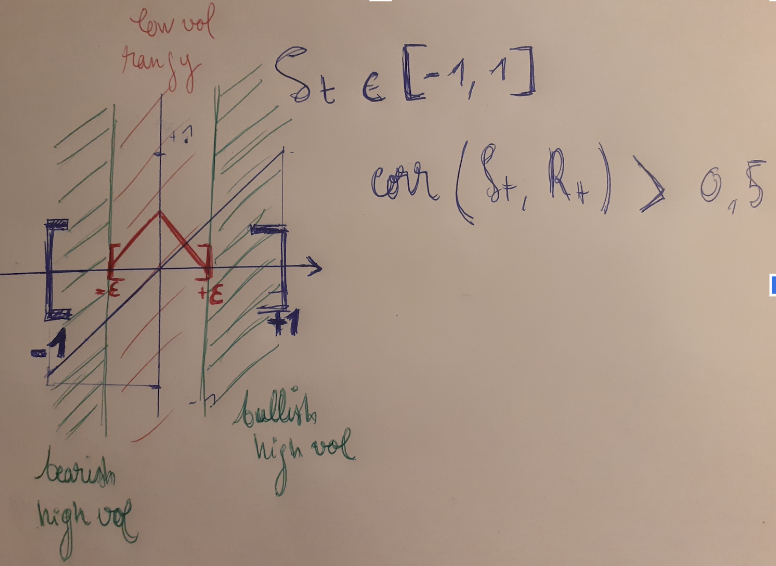
\includegraphics[scale=0.5]{Plots/signal_hourly.png}
    \caption{On/Off Liquidity provisionning signal}
    \label{fig:signal_hourly}
\end{figure}
This signal exhibits a very strong correlation to the hourly price return (60\% over 5 years).\\
The idea is to use an epsilon threshold to trigger an exit signal to discriminate the hours where we will enter liquidity and the ones where we won't (methodology described in figure \ref{fig:signal_hourly}).\\
We here display the reconstituted performance of a strategy which would be long when we will provide liquidity provision (for a signal such that $\abs(S_t)<\epsilon$) for different epsilons :
\begin{figure}[h!]
    \centering
    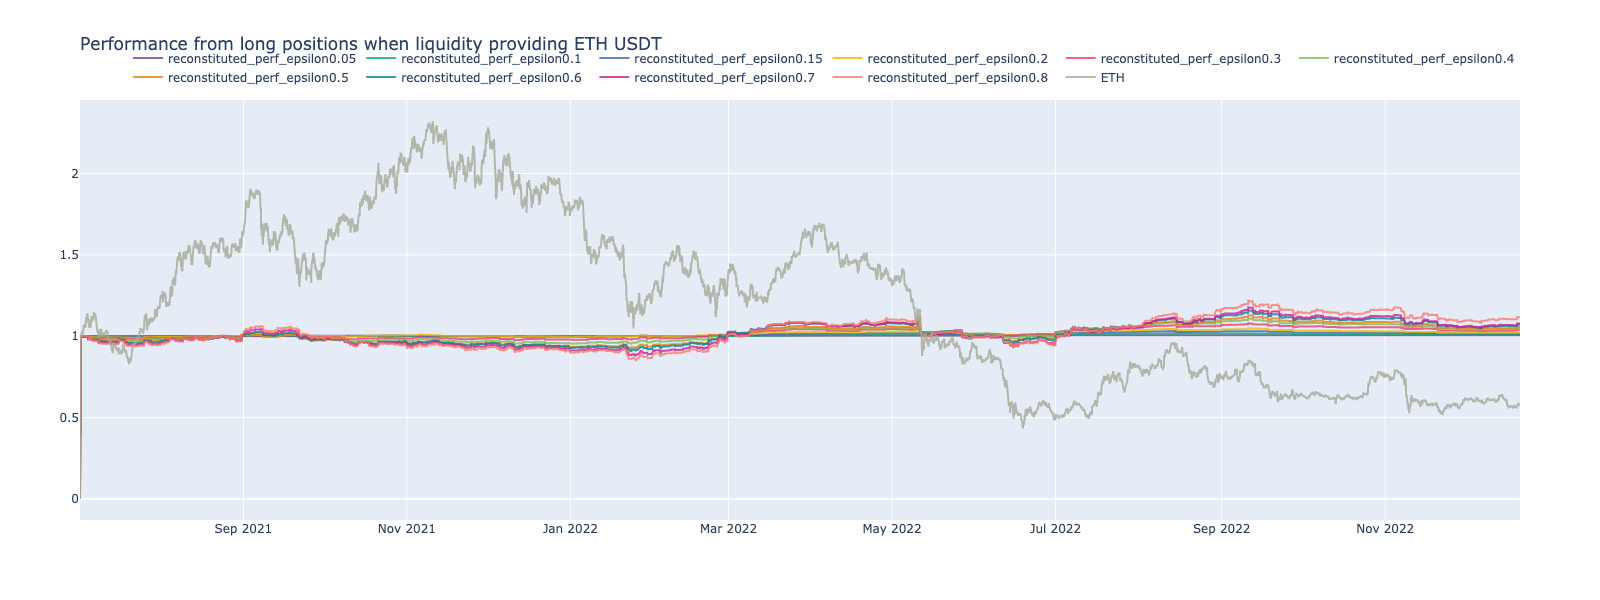
\includegraphics[scale=0.15]{Plots/signal_ETH.png}
    \caption{Rangy market capture}
    \label{fig:signal_hourly}
\end{figure}
We see the signal is making a good job at capturing rangy market.\\
\section{Modelling generated fees}
\subsection{Dex volume historical data}
We fetch the specific ETH-USDC volume on Uniswap V3 for the 0.3\% fee pool using the graph protocol.
\begin{figure}[h!]
    \centering
    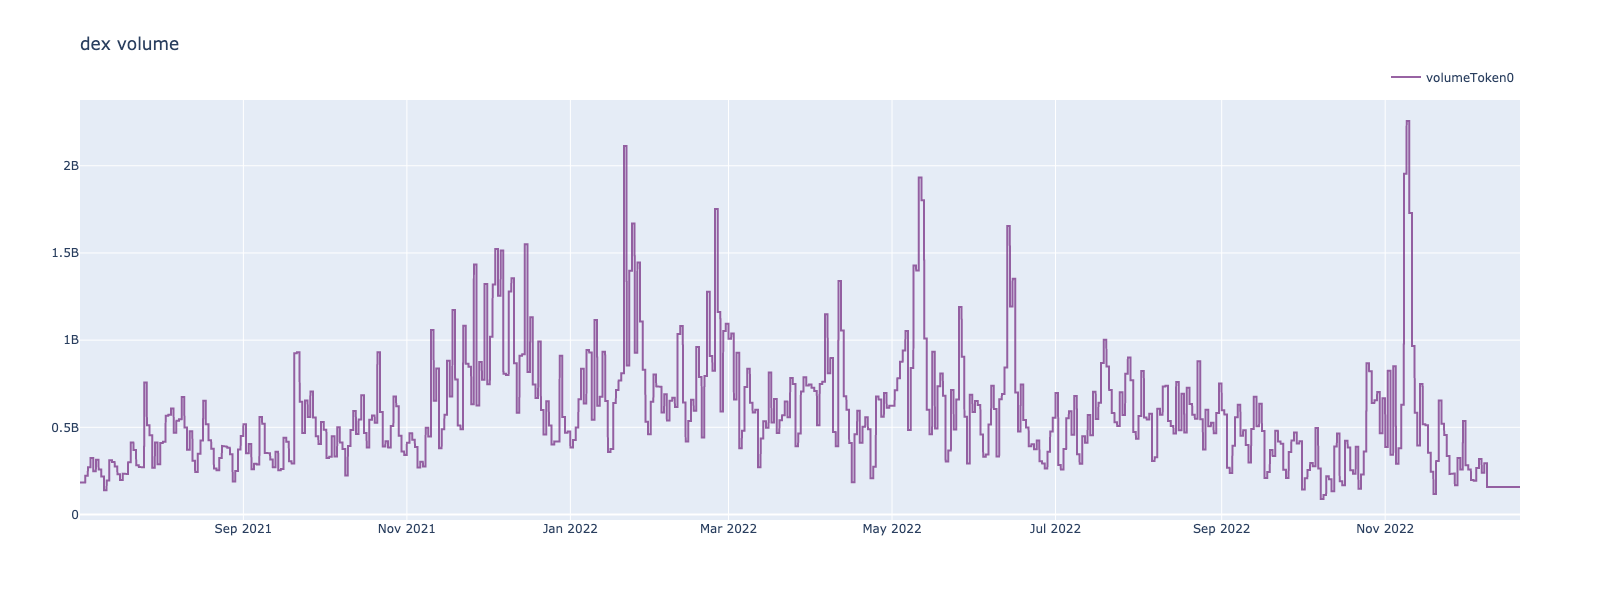
\includegraphics[scale=0.15]{Plots/dex_volume_ETH.png}
    \caption{Rangy market capture}
    \label{fig:dex_volume}
\end{figure}
\subsection{Generated fees and v3 bounds}
We take a snapshot of the APY generated by a LP position whose bounds have been placed around $x\%$ for $x$ varying between 1\% to 300\%.
\begin{figure}[h!]
    \centering
    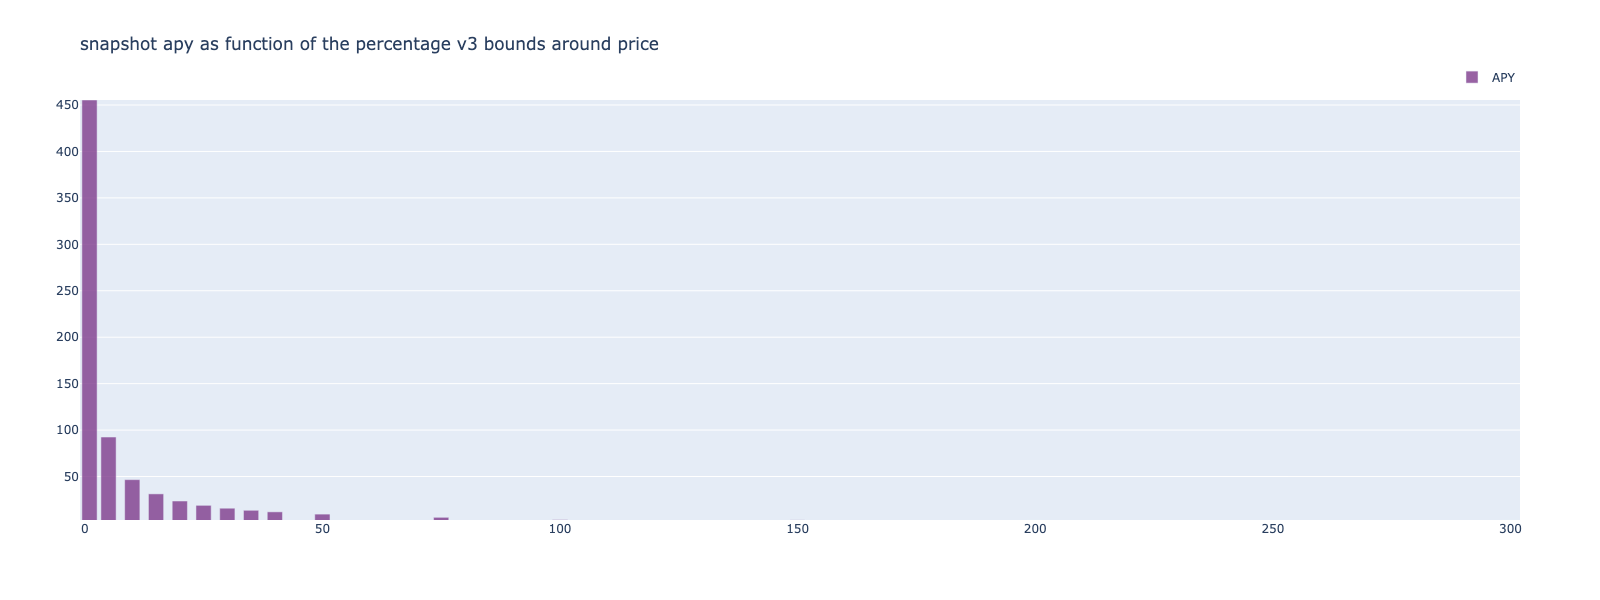
\includegraphics[scale=0.15]{Plots/apy_snapshot_ETH.png}
    \caption{Rangy market capture}
    \label{fig:apy_snapshot}
\end{figure}

\subsection{Generated fees historical data}
We then model the generated fees by a simple rule thumb of pro rata dex volume to get historical data.
\begin{equation}
APY\left(t\right) = APY\left(T\right) * \frac{DEX-VOLUME\left(t\right)}{DEX-VOLUME\left(T\right)}
\end{equation}
\begin{figure}[h!]
    \centering
    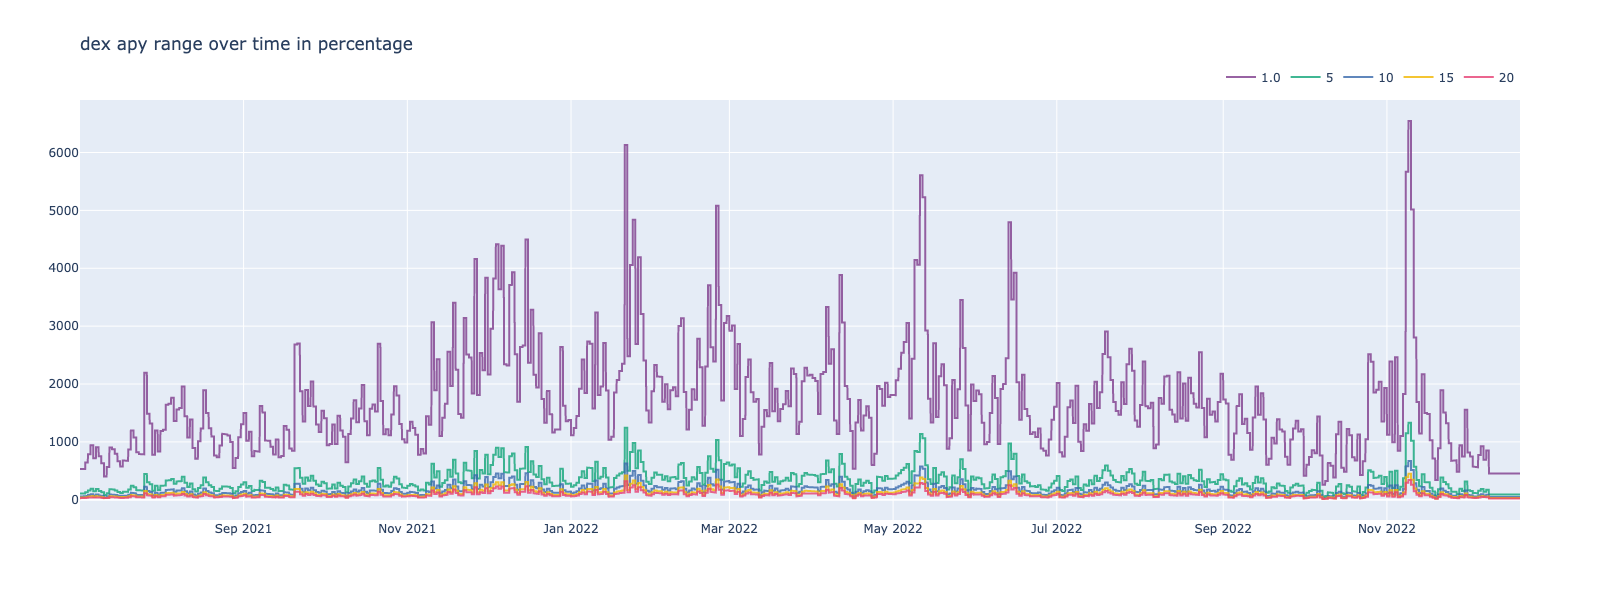
\includegraphics[scale=0.15]{Plots/apy_over_time_ETH.png}
    \caption{APY over time as a function of the v3 bound tighteness}
    \label{fig:apy_over_time}
\end{figure}
This is a necessary approximation as we can't reproduce the whole past liquidity profile.\\

\begin{description}
  \item[$\bullet$ Daily Fees = Pool Volume * Pool Fee \% * Liquidity Coverage Expected Value]
  \item[$\bullet$ APY = (Daily Fees / 1000) * 365\\]
\end{description}
Finally choose the highest APY position for each pool
\subsection{Encompassing the market by defining bounds}
The idea behind Uniswap V3 is that the user can and must specify a price range where he wants to bring the liquidity for a better capital efficiency.
\\
It also means that the procedure is not as straightforward as in Uniswap V2 and requires retail liquidity provider to have at least an opinion on the optimal bounds to choose.\\
The price range is specified by two bounds on the risky asset price $P_a <= P_b$ and the liquidity brought by the user will only account for that range allowing a huge gain in capital efficiency.\\
The tighter the bounds, the more efficient the liquidity capital is, but the more you will have to rebalance and incur impermanent loss and swapping costs.\\

The bounds are fixed by a $x\%$ distance around the initial position entering $P_0$ price.
\begin{equation}
P_b = P_0 + x*P_0
\end{equation}
\begin{equation}
P_a = P_0 - x*P_0
\end{equation}
\begin{equation}
P_0 = \frac{P_a + P_b}{2} 
\end{equation}
Getting an idea of the proper optimal $x$ is the topic of the next sections. 
\subsection{IL incurred at liquidity exit triggered}
If we were to rebalance each time a bound is reached, we can rewrite the v3 impermanent loss according to the strategy. \\
By noting $\kappa = \frac{P_b}{P_a} = \frac{P_0 + x*P_0}{P_0-x*P_0}  $, the v3 impermanent loss can be rewritten:
\begin{equation}\label{eq:ILv3Stratbis}
\frac{V_{arbitraged} - V_{held}}{V_{held}} = 
IL_{v2}(\tau)*\frac{1}{1 -\frac{ \sqrt{\frac{2}{1 +\kappa}} + \tau*\sqrt{\frac{1}{2}(1+\frac{1}{\kappa})}} { 1+\tau}}}
\end{equation}
where $\tau = \frac{P_t}{P_0}$ as defined in the appendix \ref{eq:deftau}.
Maximum incurred impermanent loss will happen if a position is exited when one of its bound is reached. Two different maximum incurred IL loss depending on whether we reached the lower bound or the upper bound.\\
Upper bound reached impermanent loss:\\
\begin{equation}
\tau_{up} = \frac{P_0+x*P_0}{P_0} > 1   
\end{equation}
Lower bound reached impermanent loss:\\
\begin{equation}
\tau_{down} = \frac{P_0-x*P_0}{P_0} < 1   
\end{equation}
Equation \ref{eq:ILv3Stratbis} and its simplified version \ref{nasty_il} shows how nasty v3 impermanent loss can be for tighter bounds.\\
But this configuration will rarely be hit, as the volatily exiting signal will most likely prevent trendy market which would lead to that case.\\
Most of the time, $P_t \approx P_0 $ resulting in a $IL \approx 0$.\\
That is the whole goal of the exiting signal.\\
\subsection{No swapping cost for the market neutral}
For huge AUM (asset under management) and fully on-chain rebalancing vaults, price slippages occurring during swaps can be very detrimental to the strategy.\\
The market neutral version has a huge advantage : no swapping will be required.\\
The asset is borrowed and liquidity will only be added/removed liquidity according to our signal.\\
\begin{figure}[h!]
    \centering
    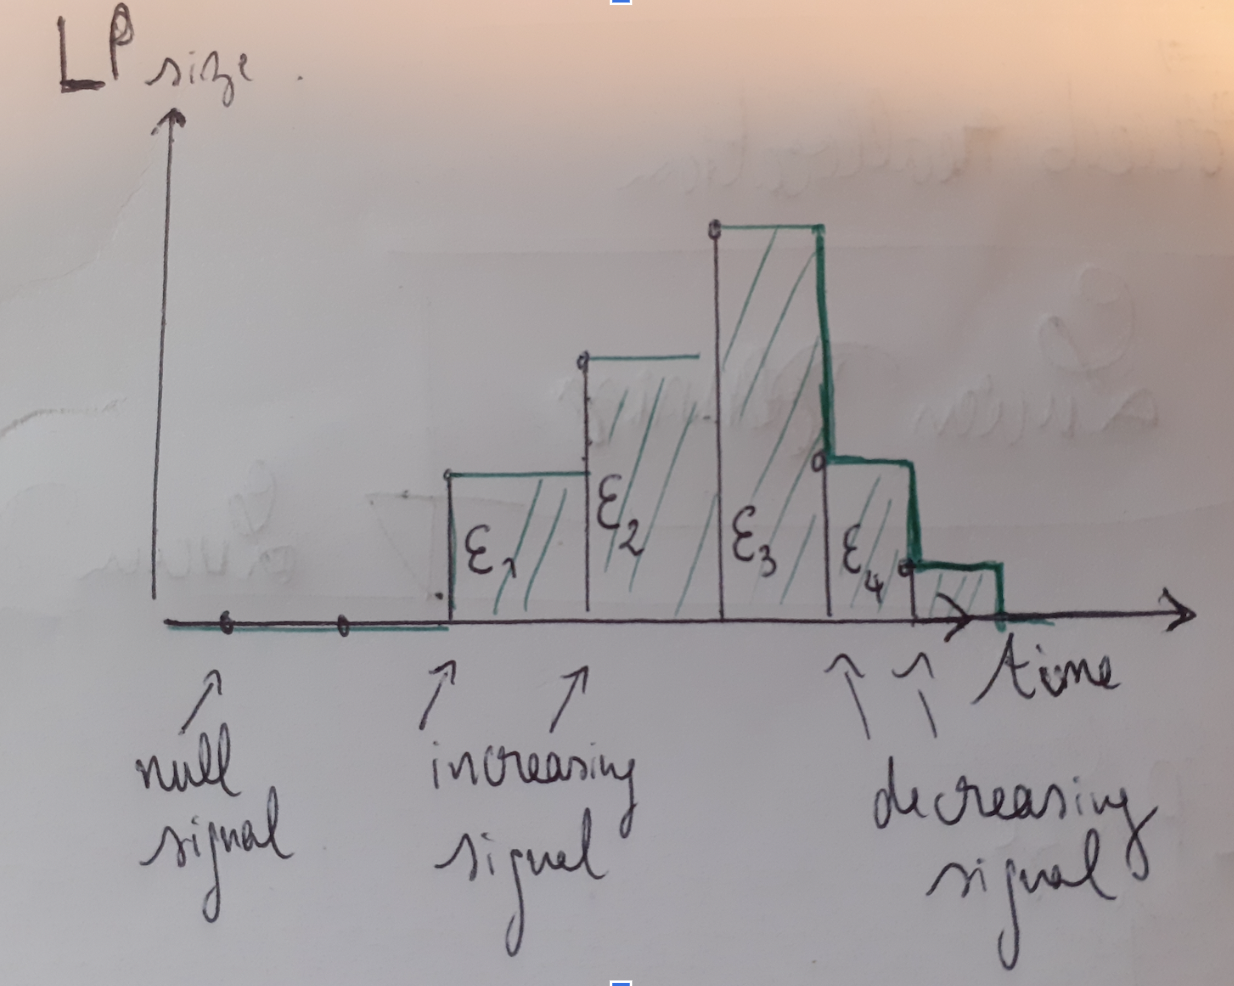
\includegraphics[scale=0.25]{Plots/lp_over_time.png}
    \caption{APY over time as a function of the v3 bound tighteness}
    \label{fig:apy_over_time}
\end{figure}

\section{Exhaustive optimization}
\subsection{Getting the optimal parameters: A trade-off between IL, transaction costs and generated LP fees}
Optimal bound distance $x$, volatility exiting signal $\epsilon$ must be calibrated for an optimal APY.
\\
\begin{description}
\item[$\bullet$]Maximize price inside the tightest bounds to earn most LP fees (the tighter the bounds, the efficienter the capital)
\item[$\bullet$]Calibrate liquidity provision signal epsilon : a small epsilon will bring very low impermanent loss but also very low LP fees as your market making time proportion will drastically drop.   \item[$\bullet$] Add/remove transaction costs have to be minimized
\end{description}
We here propose an exhaustive search of the optimal parameters by running a backtest for each configuration and choosing the solution with the best Sharpe ratio.\\
\begin{equation}
\max_{(x, epsilon)} \left[ Sharpe\left(x, epsilon\right)\right]
\end{equation}
where $Sharpe\left(x, epsilon\right)$ is the sharpe ratio of the backtested path with $x$ and $epsilon$ as specific parameters for the algorithm.

\section{Results}\label{result}
The optimal parameters chosen after an exhaustive search are :
\begin{equation}
\left\{\begin{array}{lll}
early-exit = True\\
x = 3\%\\
\epsilon = 80\%
\end{array}
\right.
\end{equation}
\subsection{Absolute performance}
\begin{figure}[h!]
    \centering
    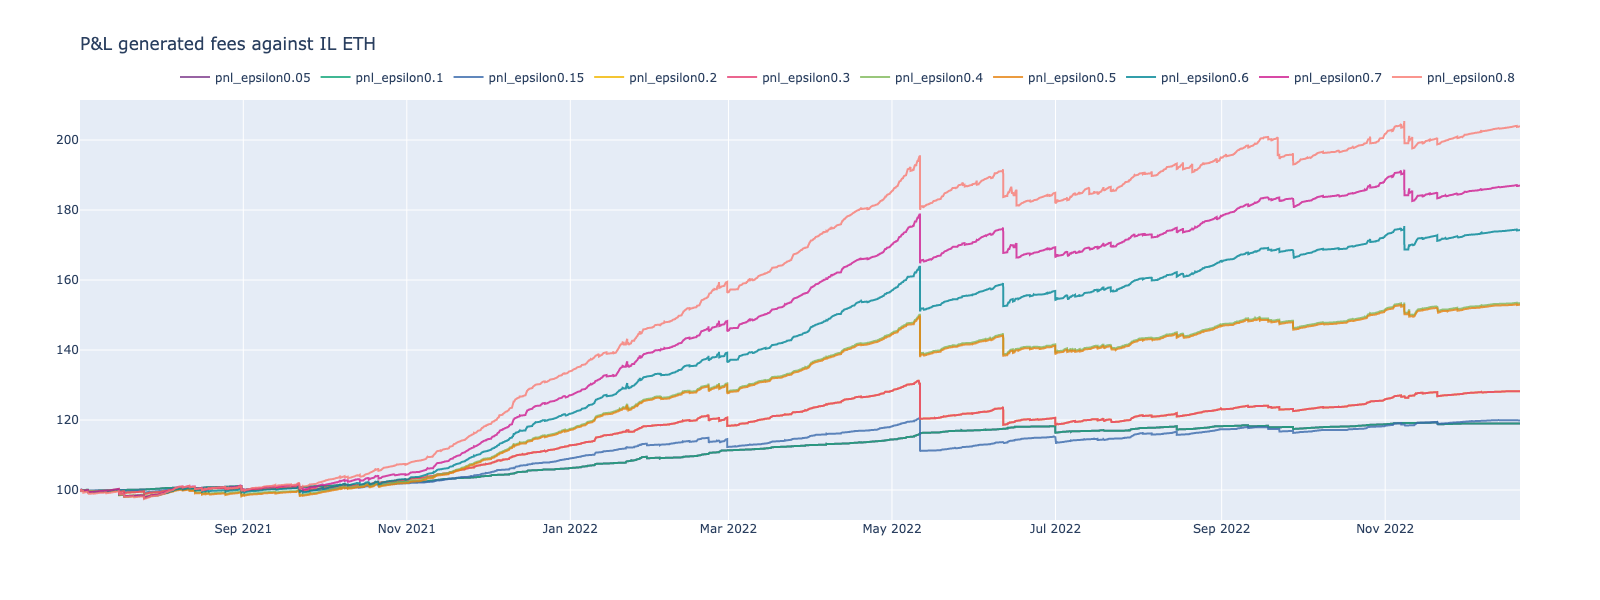
\includegraphics[scale=0.15]{Plots/PL_generated_fees_against_IL_borrow rate_transaction cost_ETH.png}
    \caption{Absolute performance}
    \label{fig:abs_perf}
\end{figure}
We here plot the absolute performance of the strategy in stable coin. \\
\begin{figure}[h!]
    \centering
    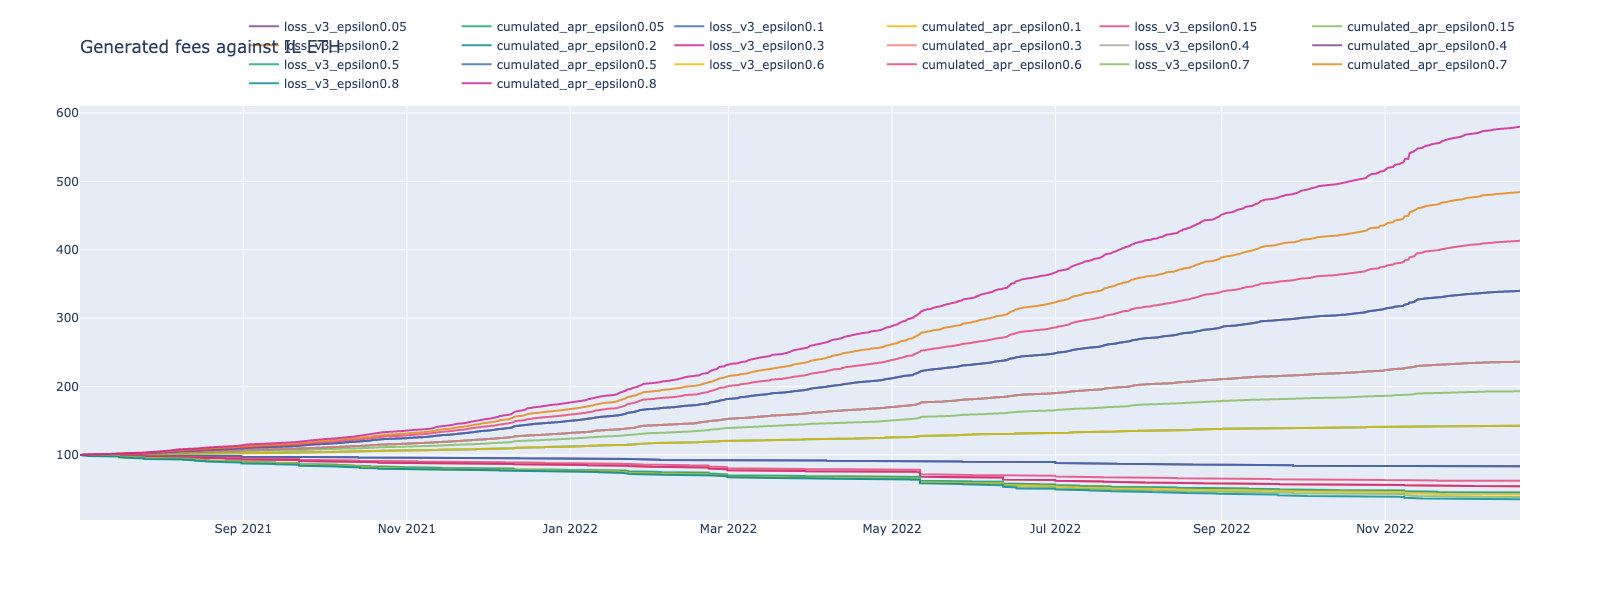
\includegraphics[scale=0.15]{Plots/Generated_fees_against_IL_ETH.png}
    \caption{Compounded generated liquidity fees versus IL v3 loss}
    \label{fig:fees_agains_apr}
\end{figure}

\begin{figure}[h!]
    \centering
    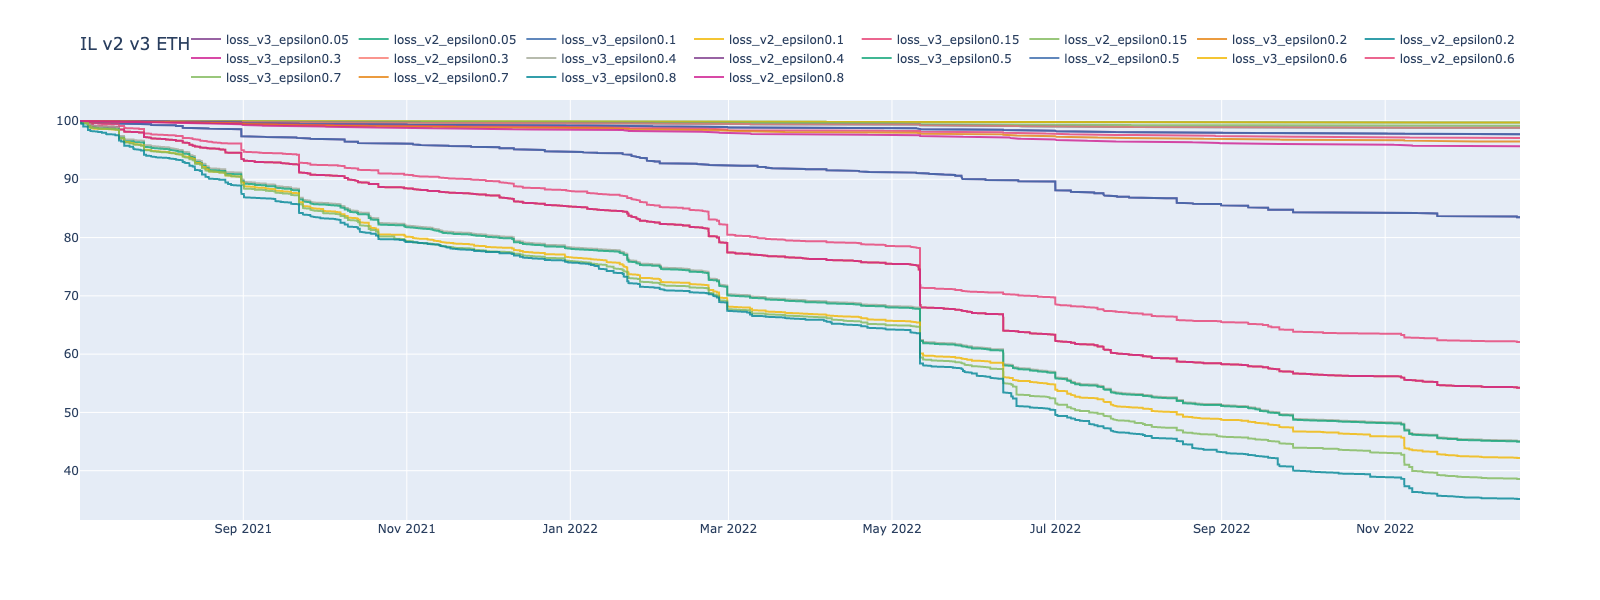
\includegraphics[scale=0.15]{Plots/IL_v2_v3_ETH.png}
    \caption{Compounded generated liquidity fees versus IL v3 loss}
    \label{fig:il_v2_v3}
\end{figure}




\section{Hedging the position}
The \ref{result} results section clearly expose that the biggest losses for that strategy in absolute performance are when the risky underlying price drops. If it drops enough to trigger a rebalancing, then we have a concurrence of impermanent loss, risky asset depreciation and swapping costs which can ruin multiple months of fees generation.\\
We therefore here propose to modulate the strategy by using proprietary trend following forecasting indicator to give a downside risk level for the epoch to come.\\
According to that indicator, we here under propose two different methodologies.


\subsubsection{Hedging with options instead of a short leg}
\subsubsubsection{Replicating the LP payoff}
We here investigate another way of mitigating our downside risk when assessing downside risky epoch.\\
We here propose to replicate the $LP$ value payoff at the end of an epoch by a basket of options whose maturity matches the end of the epoch.\\
We then optimize the options allocation to exactly fit the LP value payoff.\\

This can easily be done by an optimization algorithm minimizing the $L2$ norm between the LP payoff and the derivatives payoff.\\
We fetch from Derebit all options for a specific maturity. For each strike, we compute long/short versions of call/put payoffs:\\
\begin{equation}
\begin{array}{llll}
\text{Payoff Long Call} =  \max(0,P_f-K)\\
\text{Payoff Short Call} = -\max(0,P_f-K)\\
\text{Payoff Put Call} = \max(0,K-P_f)\\
\text{Payoff Long Call} = -\max(0,K-P_f)\\
\end{array}
\end{equation}
For a basket of weights $\theta=(\theta_i)$, we compute the final payoff:\\
\begin{equation}
Payoff(\theta, P_f) =\sum_{\theta_i in\theta}\theta_i*payoff_{\theta_i}(P_f)
\end{equation}
We then minimize the functional of the $L2$ distance between the two payoffs:
\begin{equation}
J(\theta) = \sum_{P_f in [0,+\infty[}(Payoff(\theta, P_f)-LP_{PnL}(P_f))^2
\end{equation}
This loss function can be optimized via Stochastic Gradient Descent. 
Each weight can be positive or negative. A positive value is a
long position in the options contract, while a negative value is a
short position.\\
We here under give an example of a replicated LP PnL at a one month expiry.
\begin{figure}[h!]
    \centering
    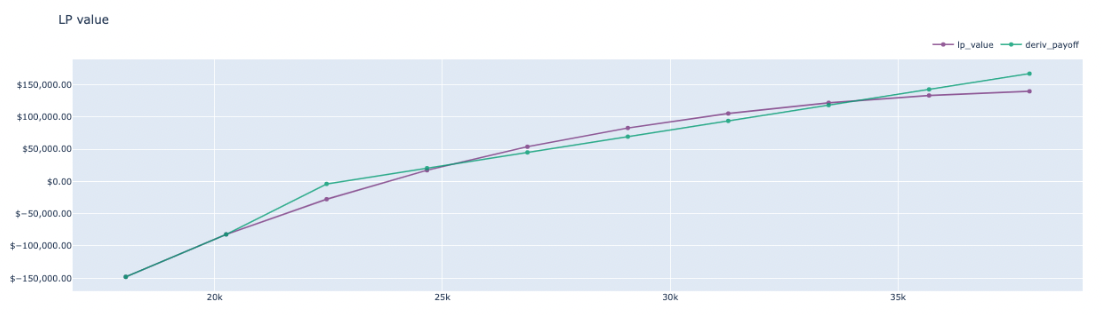
\includegraphics[scale=0.2]{Plots/option_hedging.png}
    \caption{Payoff replication using options}
    \label{fig:conc_liquidity}
\end{figure}
\subsubsubsection{Analyzing the hedging cost}
We can then analyse the total hedging cost by getting the options premium for Derebit and netting between the long and short premiums.
\begin{figure}[h!]
    \centering
    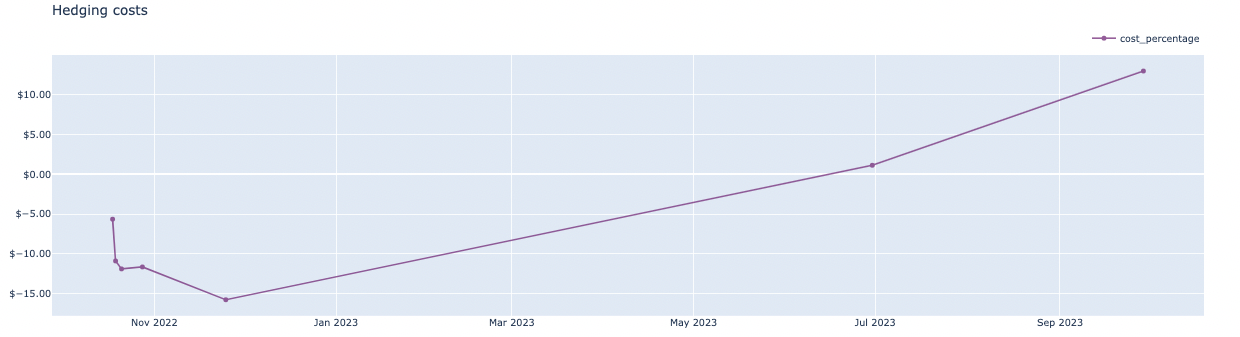
\includegraphics[scale=0.2]{Plots/hedging_costs.png}
    \caption{Hedging costs}
    \label{fig:conc_liquidity}
\end{figure}

%\section{Optimizing liquidity profile inside rangy market bounds}
%\subsection{Tick definition}
%Tick mathematical understanding is required to interpret both the values provided by the Uniswap v3 API and the data indexed %in the Uniswap v3.
%Uniswap v3 maps the continuous space of all possible prices to a discrete subset indexed by ticks.
%A tick has unique relation with price, defined by the tick base
%parameter, which is equal to 1.0001 in Uniswap (a one basis point deviation in price). The price corresponding to the i-th %tick is :
%\begin{equation}
%p(i) = {1.0001}^{i}
%\end{equation}
%However pools actually track ticks at every square root price that is an integer power of $\sqrt{1.0001}$. The tick i is %thus defined :
%\begin{equation}
%\sqrt{p(i)} = {\sqrt{1.0001}}^{i}
%\end{equation}
%\begin{equation}
%i_c = \left[\log_{\sqrt{1.0001}} \sqrt{P}\right]
%\end{equation}



\section{Conclusion}
https://medium.com/@RoboVault/delta-neutral-strategy-deep-dive-ae91d309b504
https://arxiv.org/abs/2208.03318
https://arxiv.org/pdf/2106.14404.pdf
https://uniswapv3.flipsidecrypto.com/
https://uniswaptimizer.com/
https://app.flipsidecrypto.com/velocity/queries/efed0457-5edc-46fa-ad7b-cffd01d5b93d
https://app.flipsidecrypto.com/velocity/queries/bb47119b-a9ad-4c59-ac4d-be8c880786e9
https://arxiv.org/pdf/2106.12033.pdf
https://medium.com/auditless/impermanent-loss-in-uniswap-v3-6c7161d3b445 
\appendix
\section{Understanding the risk of hyperbolic dexes (decentralized exchanges)}
\subsection{Hyperbolic equation}
Let $X$ denote the reserve of the risky asset (Ether, WBtc, SOL) and $Y$
denote the reserve of the non risky stable coin (USDT, USDC, BUSD, ..).
Uniswap pioneering approach was to force the reserve quantities on the pool to live on an hyperbole, hence the denomination hyperbolic dex.
\begin{equation}
    X * Y = cte = X_{t0} * Y_{t0}
\end{equation}
The constant is fixed by the initially brought amount at instant $t0$.
The risky asset price $X$ in stable coins $Y$ is directly linked to the pool reserve:
\begin{equation}
    P_{X \text{ in }Y}  = \frac{Y}{X} = P_X
\end{equation}
Basically if you have one Ether (X = 1) and 4500 USDT in the pool (Y = 4500), the ether
price is $\frac{4500}{1}$. And vice versa
\begin{equation}
    P_{Y \text{ in }X}  = \frac{X}{Y} = P_Y
\end{equation}
By denoting $L^2 = X_{t0} * Y_{t0}$ (L can be seen as the part of the liquidity brought by a single asset of the pool), a quick computation gives:
\begin{equation}
    L=\sqrt{X*Y}
\end{equation}
\begin{equation}
    X = \frac{L}{\sqrt{P_X}}  
\end{equation}
\begin{equation}
    Y = L*\sqrt{P_X}
\end{equation}

\subsection{Uniswap V2 Impermanent loss}
Uniswap V2 liquidity pools  are actively managed by arbitraging bots/traders which swap
the proper quantities to readjust the pool quantities to match the consensus price formed over all exchanges (centralized and decentralized).\\
Let's denote $t_1$ an instant where the pool quantities are denoted $X_{t_1}$, $Y_{t_1}$, $P_{X,t_1}$, $P_{Y,t_1}$.
Let's denote $t_2 > t_1$ a subsequent instant where the pool quantities are denoted $X_{t_2}$, $Y_{t_2}$, $P_{X,t_2}$, $P_{Y,t_2}$.

Let's imagine two different states of the reality. A first one where the pool has not been arbitraged and a second one where the pool has been arbitraged.

The quantities at instant $t_2$ when the pool has been arbitraged match the consensus price $P_{consensus}$:
\begin{equation}
    P_{X_{t_2}} = \frac{Y_{t_2}}{X_{t_2}} = P_{consensus}
\end{equation}

If the pool has not been arbitraged, its reserve quantities have not moved : they stayed at $X_{t_1}$, $Y_{t_1}$, $P_{X,t_1}$, $P_{Y,t_1}$.
\begin{equation}
    P_{X_{t_1}} = \frac{Y_{t_1}}{X_{t_1}}  \neq P_{consensus}
\end{equation}

Both state values of the pool in stable coins Y can be expressed as :
\begin{equation}
    V_{t_1} = X_{t_1}*P_{consensus} + Y_{t_1} = X_{t_1}*P_{X_{t_2}} + Y_{t_1}
\end{equation}
\begin{equation}
    V_{t_2} = X_{t_2}*P_{consensus} + Y_{t_2} = X_{t_2}*P_{X_{t_2}} + Y_{t_2}
\end{equation}
A quick computation gives the impermanent loss formula (the risk of loss for a non
arbitraged pool whose risky asset price has moved :
\begin{equation}
    \frac{v_{t_2} - v_{t_1}}{v_{t_1}} = \frac{2*\sqrt{\frac{P_{X_{t_2}}}{P_{X_{t_1}}}}}{1+\frac{P_{X_{t_2}}}{P_{X_{t_1}}}}-1
    =\frac{2*\sqrt{P_{X_{t_1}}P_{X_{t_2}}} - (P_{X_{t_1}} + P_{X_{t_2}}) } {P_{X_{t_1}} + P_{X_{t_2}}}
\end{equation}
This function is symmetrical in $P_{X_1}$ the price of the non-arbitraged pool at instant $t1$ and $P_{consensus} = P_{X_2}$ the consensus price at $t2$.
\\
The proof is straightforward :
$$
    \frac{v_{t_2} - v_{t_1}}{v_{t_1}} =     \frac{\frac{v_{t_2} - v_{t_1}}{X_{t_1}}} {\frac{v_{t_1}}{X_{t_1}}} = \frac{\frac{v_{t_2}}{X_{t_1}} - (P_{X_{t_1}} + P_{X_{t_2}})} {P_{X_{t_1}} + P_{X_{t_2}}}
$$
because $\frac{v_{t_1}}{X_{t_1}} = P_{X_{t_1}} + P_{X_{t_2}$.
$$
\frac{v_{t_2}}{X_{t_1}} =\frac{X_{t_2}*P_{X_{t_2}} + Y_{t_2}}{X_{t_1}} 
$$
$$
\frac{v_{t_2}}{X_{t_1}} ==\frac{2*Y_{t_2}}{X_{t_1}} =\frac{2*L*\sqrt{P_X_{t_2}}}{X_{t_1}}
$$
$$
\frac{v_{t_2}}{X_{t_1}} =\frac{2*L*\sqrt{P_X_{t_1}P_X_{t_2}}}{P_X_{t_1} * X_{t_1}} 
$$
$$
\frac{v_{t_2}}{X_{t_1}} =\frac{2*L*\sqrt{P_X_{t_1}P_X_{t_2}}}{\sqrt{P_X_{t_1}} * X_{t_1}} = 2* \sqrt{P_X_{t_1}P_X_{t_2}}
$$

By renaming $\frac{P_{X_{t_2}}}{P_{X_{t_1}}} = \tau $
We can rewrite the impermanent loss equation :
\begin{equation}
    \frac{v_{t_2} - v_{t_1}}{v_{t_1}} = \frac{2*\sqrt{\tau}}{1+\tau}}-1 = IL_{v2}(\tau)
\end{equation}
\begin{figure}[h!]
    \centering
    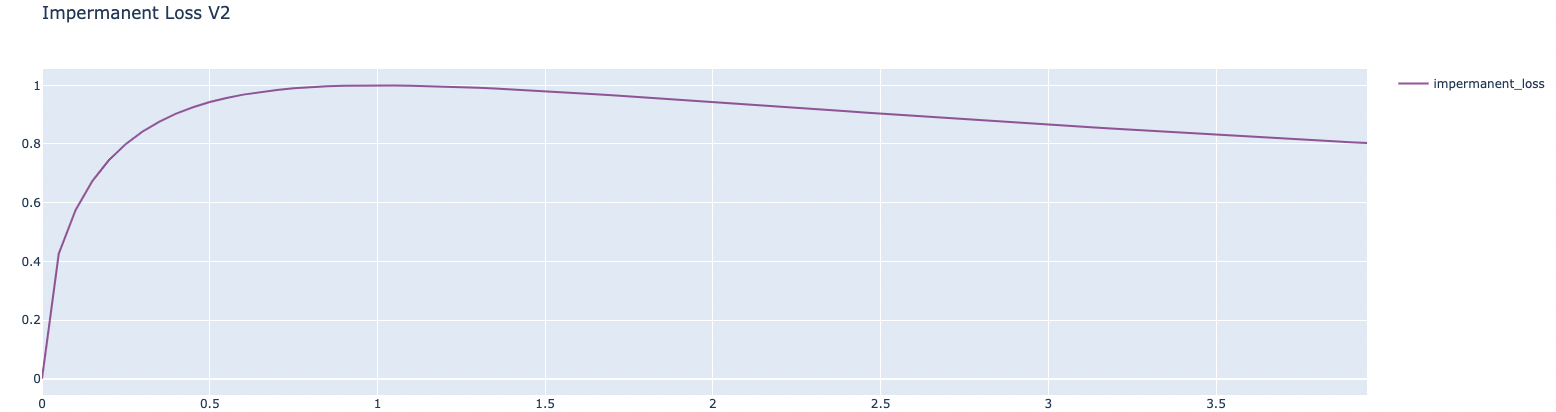
\includegraphics[scale=0.15]{Plots/impermanent_loss.png}
    \caption{Impermanent loss versus price ratio}
    \label{fig:rangy_market}
\end{figure}

\begin{description}
\item[$\bullet$1.25x price change results in a 0.6\% loss relative to HODL]
\item[$\bullet$1.50x price change results in a 2.0\% loss relative to HODL]
\item[$\bullet$1.75x price change results in a 3.8\% loss relative to HODL]
\item[$\bullet$2x price change results in a 5.7\% loss relative to HODL]
\item[$\bullet$3x price change results in a 13.4\% loss relative to HODL]
\item[$\bullet$4x price change results in a 20.0\% loss relative to HODL]
\item[$\bullet$5x price change results in a 25.5\% loss relative to HODL]
\end{description}
“N.B. The loss is the same whichever direction the price change occurs in  (doubling in price results in the same loss as halving).\\

\subsection{Uniswap V3 Impermanent loss}
The idea behind Uniswap V3 is that the user can specify a price range where he wants to bring the liquidity.
\\
The price range is specified by two bounds on the risky asset price $P_a <= P_b$ and the liquidity brought by the user will only account for that range allowing a huge gain in capital efficiency.\\


\subsubsection{Capital efficiency and uniswap v3}
From now on, the only price we will deal with is the price of the risky asset in stable coin.
\begin{equation}
    P = P_X = P_{X \text{ in }Y}  = \frac{Y}{X}
\end{equation}
With that notation, it comes :
\begin{equation}
    L=\sqrt{X*Y}
\end{equation}
\begin{equation}
    X = \frac{L}{\sqrt{P}}  
\end{equation}
\begin{equation}
    Y = L*\sqrt{P}
\end{equation}
\subsubsection{ Swapping inside a tick}
Inside a tick, everything works as with the previous Uniswap V2 protocol with virtual reserves.
\begin{equation}
    X_{virtual} * Y_{virtual} = L^2
\end{equation}
And the reserves evolution are dictated by
\begin{equation}
   \Delta \sqrt{P} = \frac{\Delta Y}{L}
\end{equation}
\begin{equation}
   \Delta \frac{1}{\sqrt{P}} = \frac{\Delta X}{L}
\end{equation}
The smart contract will only track the $L$ and $\sqrt{P}$. The reserve will be updated
accordingly.

\\
The risky asset reserve matching the highest price for which the liquidity provider is ready to provide liquidity :
\begin{equation}
    X_b = \frac{L}{\sqrt{P_b}}
\end{equation}
The stable coin reserve matching the lowest price for which the liquidity provider is ready to provide liquidity :
\begin{equation}
    Y_a = L *\sqrt{P_a}
\end{equation}
\begin{equation}
\left\{
\begin{array}{ll}
  X_{virtual} = X_{real}+\frac{L}{\sqrt{P_b}}\\
  Y_{virtual} = Y_{real} + L *\sqrt{P_a}\\
\end{array}
\right.
\end{equation}
The hyperbole equation thus becomes:
\begin{equation}
    (X_{real}+\frac{L}{\sqrt{P_b}})* (Y_{real} + L *\sqrt{P_a})= L^2
\end{equation}
From now on, we will give up the real tag and call $X=X_{real}$ and $Y=Y_{real}$.
%For $P\ge P_b$:
%\begin{equation}
%\left\{
%\begin{array}{ll}
%X=0\\
%Y=L*(\sqrt{P_b}-\sqrt{P_a})\\
%\end{array}
%\right.
%\end{equation}
%\\
%For $P\le P_a$:
%\begin{equation}
%\left\{
%\begin{array}{ll}
%X=L*\frac{\sqrt{P_b}-\sqrt{P_a}}{\sqrt{P_b}*\sqrt{P_a}}\\
%Y=0\\
%\end{array}
%\right.
%\end{equation}
%\\
%For $P_a \le P \le P_b $:
%\begin{equation}
%\left\{
%\begin{array}{ll}
%X=X_{virtual}-\frac{L}{\sqrt{P_b}}=L*(\frac{1}{\sqrt{P}}-\frac{1}{\sqrt{P_b}}) %=L*\frac{\sqrt{P_b}-\sqrt{P}}{\sqrt{P_b}*\sqrt{P}}\\
%Y=Y_{virtual}-L*\sqrt{P_a}\ = L*(\sqrt{P}-\sqrt{P_a})\\
%\end{array}
%\right.
%\end{equation}
\\
The solution is given by the three different regimes according to the current price $P$ location regarding the liquidity bounds:
\begin{equation}\label{three_regime}
\left\{
\begin{array}{cc}
\begin{array}{lllll}
\left\{
\begin{array}{ll}
X=0\\
Y=L*(\sqrt{P_b}-\sqrt{P_a})\\
\end{array}
\right. & ,P\ge P_b\\
& \\
\left\{
\begin{array}{ll}
X=L*(\frac{1}{\sqrt{P}}-\frac{1}{\sqrt{P_b}}) \\
Y= L*(\sqrt{P}-\sqrt{P_a})\\
\end{array}
\right.&  ,P_a \le P \le P_b \\
&\\
\left\{
\begin{array}{ll}
X=L*(\frac{1}{\sqrt{P_a}}-\frac{1}{\sqrt{P_b}})\\
Y=0\\
\end{array}
\right.& ,P\le P_a\\
\end{array}
\right.\\
\end{array}
\end{equation}

\begin{figure}[h!]
    \centering
    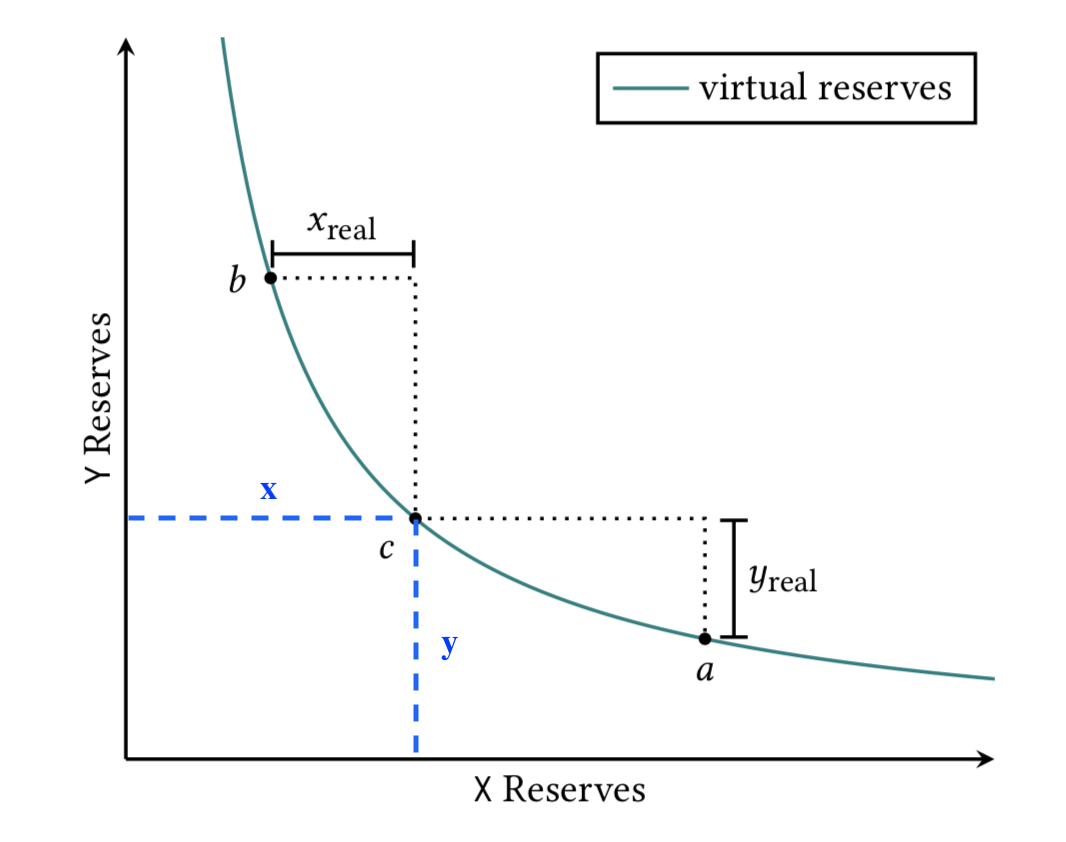
\includegraphics[scale=0.2]{Plots/concentrated_liquidity.png}
    \caption{Concentrated liquidity between a and b}
    \label{fig:conc_liquidity}
\end{figure}
\subsection{Computing the impermanent loss}
The value of the pool at a time $t$ when the pool is arbitraged :
\begin{equation}
V=X*P+Y\\
\end{equation}
$$
V = L*( \frac{1}{\sqrt{P}}-\frac{1}{\sqrt{P_b}})*P + L*(\sqrt{P}-\sqrt{P_a})
$$
\begin{equation}
V = 2*L*\sqrt{P}-L*(\sqrt{P_a}+ \frac{P}{\sqrt{P_b}}})
\end{equation}

Let's define $P_{consensus}$, the new price coming from a market consensus and $\tau>0$ the price ratio.
\begin{equation}\label{eq:deftau}
P_{consensus} = \tau*P\\
\end{equation}

The value of the arbitraged pool with the new consensus price is then :
\begin{equation}
V_{arbitraged} = 2*L*\sqrt{\tau*P}-L*(\sqrt{P_a}+ \frac{\tau*P}{\sqrt{P_b}}} )
\end{equation}

\begin{equation}
V_{held} = X*P_{consensus}+Y
\end{equation}
$$
V_{held} = L*( \frac{1}{\sqrt{P}}-\frac{1}{\sqrt{P_b}})*P_{consensus}+L*(\sqrt{P}-\sqrt{P_a})+ \\
$$

$$
V_{held} = L*\sqrt{P}*(1+\tau)-L*(\sqrt{P_a}+ \frac{\tau*P}{\sqrt{P_b}}})\\
$$
The V3 impermanent loss is thus after a quick computation :
\begin{equation}\label{eq:ILv3}
\frac{V_{arbitraged} - V_{held}}{V_{held}} = 
IL_{v2}(\tau)*\frac{1}{1 -\frac{ \sqrt{\frac{P_a}{P}} + \tau*\sqrt{\frac{P}{P_b}}} { 1+\tau}}} = IL_{P_a,P_b}(\tau)
\end{equation}
where $IL_{v2}(\tau)=\frac{2*\sqrt{\tau}}{1+\tau}}-1 = IL_{v2}(\tau)$ is the standard uniswap V2 impermanent loss for the range $\left[0,+\infty\right[$.\\
In the case $P_a = P_b = P$, then the impermanent loss will be $0$.
\begin{equation}
\lim\limits_{P_a \to 0, P_b \to +\infty} IL_{P_a,P_b}(\tau) = IL(\tau)
\end{equation}
When the liquidity bounds are pushed to $[0,+\infty[$, the $v3$ impermanent loss goes back to the original v2 one.\\
 
Finally, setting $\tau$ to 1, we do get 0 since there should not be any impermanent loss in any scenario, v2 or v3.\\
\subsubsection{V3 Impermanent loss is larger}\label{v3isbad}
If we take the simple assumption $p_a = \frac{P}{n}$ and $p_b = n*P$, we get the following loss :
\begin{equation}\label{nasty_il}
IL_{P_a,P_b}(\tau) = IL(\tau) * \frac{1}{1-\frac{1}{\sqrt{n}}}
\end{equation}
\begin{figure}[h!]
    \centering
    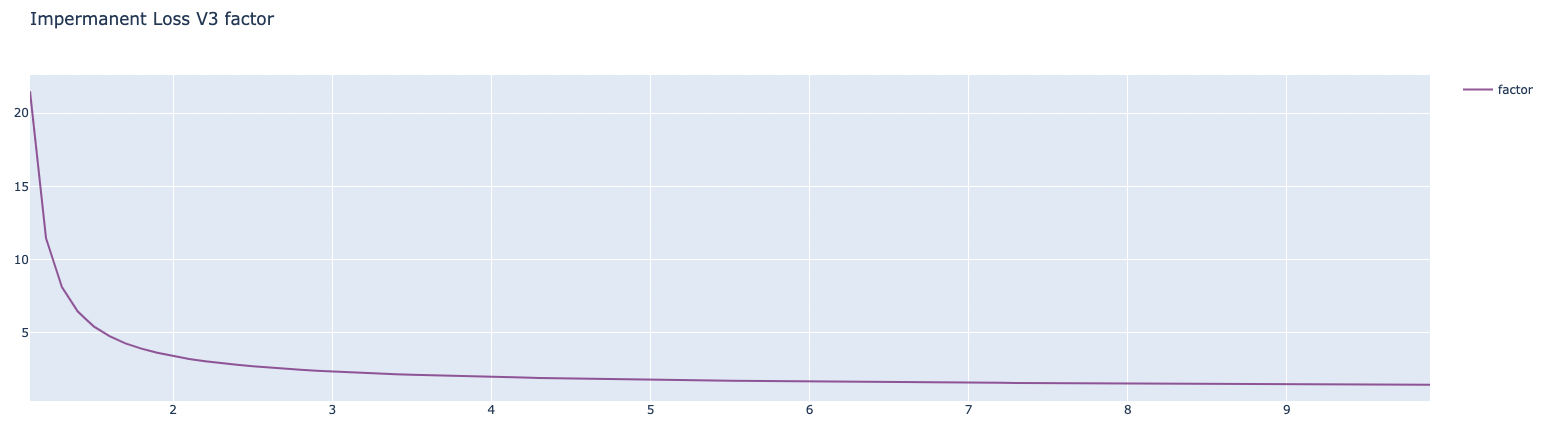
\includegraphics[scale=0.15]{Plots/factor.png}
    \caption{Impermanent loss V3 factor}
    \label{fig:rangy_market}
\end{figure}

Even if our liquidity range is big enough to accommodate prices doubling or halving, impermanent loss is nearly 4 times higher than if we provided liquidity in the whole range of prices.\\
And that is excluding the impermanent loss associated with falling outside the concentrated liquidity range.\\
\subsection{Uniswap V3 LP liquidity providing value}
\subsubsection{Add/deletion of liquidity}
When adding or removing liquidity from a position, the amount of assets to add according to the amount of added liquidity $\Delta L$
is given by the equivalent formula as \ref{three_regime}:
\begin{equation}\label{liquidity_adding}
\left\{
\begin{array}{cc}
\begin{array}{lllll}
\left\{
\begin{array}{ll}
\Delta X=0\\
\Delta Y=\Delta L*(\sqrt{P_b}-\sqrt{P_a})\\
\end{array}
\right. & ,P\ge P_b\\
& \\
\left\{
\begin{array}{ll}
\Delta X=\Delta L*(\frac{1}{\sqrt{P}}-\frac{1}{\sqrt{P_b}}) \\
\Delta Y= \Delta L*(\sqrt{P}-\sqrt{P_a})\\
\end{array}
\right.&  ,P_a \le P \le P_b \\
&\\
\left\{
\begin{array}{ll}
\Delta X=\Delta L*(\frac{1}{\sqrt{P_a}}-\frac{1}{\sqrt{P_b}})\\
\Delta Y=0\\
\end{array}
\right.& ,P\le P_a\\
\end{array}
\right.\\
\end{array}
\end{equation}
\subsubsection{Valuing a liquidity position}
The initial amount of tokens $X_0$, $Y_0$ and $L$ when entering a LP position with bounds $P_a$ and $P_b$ and initial price $P_0$ will follow \ref{three_regime}.\\
You can deduct $L$ value from \ref{three_regime} applied to $X_0$, $Y_0$ and $P_0$.\\
The final amount of tokens $X$, $Y$ and $L$ when exiting a LP position with bounds $P_a$ and $P_b$ and current price $P$ will also follow \ref{three_regime} for the previous $L$.\\
The liquidity position P&L can be written as :
\begin{equation}\label{PnL}
PnL = \frac{X* P + Y}{X_0 * P_0 + Y_0} - 1
\end{equation}
\bibliographystyle{IEEEtranN}
\bibliography{bib}
\nocite{*}
\end{document}

% to do
% Expliquer l'importance de la réduction de dimension dans ML
% Expliquer la diff CCA PCA pour ML